\section{Εργαλεία}
\label{section:tools}

Στην τελευταία υποενότητα αυτού του κεφαλαίου θα μιλήσουμε για τα εργαλεία που χρησιμοποιήθηκαν
για την υλοποίηση του συστήματος Αυτόματης Παρακολούθησης που υλοποιήσαμε στο πλαίσιο της διπλωματικής
αυτής εργασίας.

\subsection{Node.js}
\label{subsec:nodejs}

Είναι ένα περιβάλλον εκτέλεσης (runtime) της προγραμματιστικής γλώσσας JavaScript.
Πληθώρα μηχανικών λογισμικού το χρησιμοποιούνε σήμερα, για την γρήγορη και, σχετικά με άλλα εργαλεία,
εύκολη ανάπτυξη διαδικτυακών εφαρμογών. Η Node.js μάλιστα διαθέτει το δικό της package manager
(ΝPM - Node Package Manager), στον οποίο διαρκώς προστίθενται καινούργιες βιβλιοθήκες
από χρήστες για χρήστες. 

Είναι σχεδιασμένο για να μπορεί να χτίζει κλιμακούμενες (scalable) εφαρμογές, καθώς η αρχιτεκτονική του,
επιτρέπει τη σύνδεση πολλών εξωτερικών συστημάτων/χρηστών και την εξυπηρέτηση αυτών ταυτόχρονα. Κάθε φορά που γίνεται κάποια σύνδεση στην εφαρμογή και κατεπακόλουθω
κάποιο αίτημα στο σύστημα εκτελείται μία callback συνάρτηση προκειμένου να μπορέσει να απαντήσει πίσω.
Όσο το σύστημα δεν δέχεται αιτήματα "κοιμάται" και περιμένει το επόμενο που θα έρθει.

Όλα όσα προαναφέρθηκαν την καθιστούν κατάλληλη για τη δημιουργία συστημάτων server. Αξίζει να σημειωθεί μάλιστα ότι για το σκοπό
αυτό υπάρχουν πλήθος βιβλιοθηκών που παρέχουν έτοιμες συναρτήσεις και διεπαφές που κάνουν την διαδικασία ανάπτυξης ακόμα πιο εύκολη
και γρήγορη. Πολλές φορές μάλιστα, κάποιες βιβλιοθήκες πέρα από βοηθητικές συναρτήσεις και υπορουτίνες, επηρεάζουν τον τρόπο
σύγγραφής κώδικα, μέσα από APIs που παρέχουν. Αυτές χαρακτηρίζονται ως frameworks, και επιταχύνουν τόσο τη διαδικασία
ελέγχου (testing), όσο και τη διαδικασία ανάπτυξης (development) του λογισμικού. Μερικές από τα πιο γνωστά
backend framerworks είναι τα: Express, Jest, Koa, Socket.io, Meteor, Loopback

Τα παραπάνω σε συνδυασμό με το ότι η JavaScript είναι μία ευρέως διαδεδομένη και πολυχρησιμοποιούμενη γλώσσα
προγραμματισμού στο διαδίκτυο δίνει την ευκαιρία σε developers να αναπτύξουν μία εφαρμογή πλήρως
(frontend και backend) με τη χρήση ενός κοινού εργαλείου. Ένα τυπικό παράδειγμα εφαρμογής που μπορεί να
αναπτυχθεί με τον τρόπο αυτό φαίνεται στο \autoref{fig:nodejs_system}.

\begin{figure}[!ht]
	\centering
	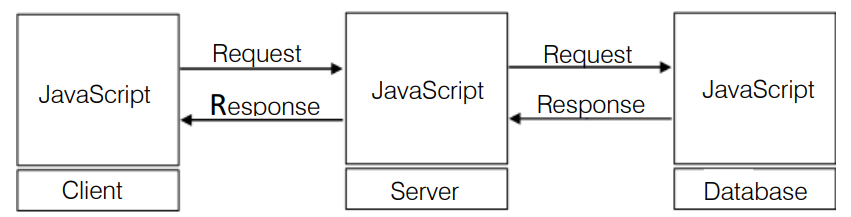
\includegraphics[width=0.8\textwidth]{./images/chapter2/javascript_end_to_end.png}
	\caption[Σχεδίαση συστήματος με χρήση Node.js]{Σχεδίαση συστήματος με χρήση Node.js \cite{nodejs_challenges_in_implementation}}
	\label{fig:nodejs_system}
\end{figure}

\subsection{PM2}
\label{subsec:pm2}

Η διαχείρηση διεργασιών (processes) που τρέχουν σε ένα υπολογιστικό σύστημα μπορεί να είναι δύσκολη
και αρκετά περίπλοκη για κάποιον που δεν διαθέτει μεγάλη πείρα σε αυτό τον τομέα. Το PM2 ή αλλιώς Process Manager 2,
αποτελεί ένα open source πρότζεκτ που κάνει την παραπάνω διαδικασία πιο απλή και κατανοητή, κερδίζοντας χρόνο
για τον developer που μπορεί να τον αξιοποιήσει για την ανάπτυξη εφαρμογών.

Με την έννοια διαχείρηση διεργασιών, αναφερόμαστε σε όλες εκείνες τις ενέργειες που σχετίζονται
με τον (πρόωρο ή όχι) τερματισμό και την παρακολούθηση ήδη υπάρχοντων διεργασιών (\autoref{fig:pm2_monitoring}), αλλά και τη δημιουργία καινούργιων.
Προγράμματα όπως το pm2 προσφέρουν ακόμα δυνατότητες όπως είναι η αυτόματη επανεκκίνηση διεργασιών σε περίπτωση σφάλματος
αποτρέποντας έτσι την ύπαρξη downtime των εφαρμογών που τρέχουμε.

Ένα από τα πιο χρήσιμα εργαλεία που παρέχει το PM2 είναι η λειτουργία cluster mode.
Αν και δεν αναφέρθηκε πιο πάνω ο συγκεκριμένος διαχειριστής διεργασιών εξειδικεύεται σε Node.js
εφαρμογές και στη διαχείρηση αυτών. Εξ ορισμού εφαρμογές γραμμένες σε JavaScript τρέχουν σε ένα thread
στο υπολογιστικό σύστημα που εκτελούνται. Χρησιμοποιώντας όμως το cluster mode, μπορούμε να
ξεκινήσουμε πολλαπλές διεργασίες που θα λειτουργούν ταυτόχρονα και θα μοιράζουν το φόρτο
κατάλληλα (load-balancing) ώστε το τελικό σύστημα να έχει καλύτερη απόδοση και να μπορεί να εξυπηρετεί 
περισσότερο κόσμο. 

\begin{figure}[!ht]
	\centering
	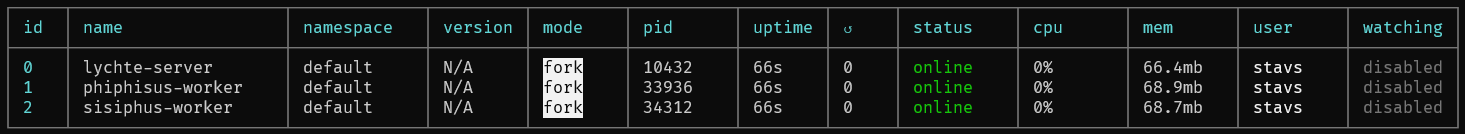
\includegraphics[width=1\textwidth]{./images/chapter2/pm2_monitoring.png}
	\caption[Παράδειγμα Παρακολούθησης διεργασιών με τη χρήση του PM2]{Παράδειγμα Παρακολούθησης διεργασιών με τη χρήση του PM2}
	\label{fig:pm2_monitoring}
\end{figure}

\subsection{MongoDB}
\label{subsec:mongodb}

H MongoDB αποτελεί μία Μη Σχεσιακή Βάση Δεδομένων (Non Relational Database), που χρησιμοποιεί documents,
για να αποθηκεύσει πληροφορία, αντί στήλες και γραμμές όπως θα είχαμε σε κλασσικές SQL βάσεις δεδομένων.
Είναι σχεδιασμένη για αποθήκευση δεδομένων μεγάλης κλίμακας και παράλληλη επεξεργασία δεδομένων μοιρασμένα
σε έναν μεγάλο αριθμό από servers. 

Τα documents που αναφέρθηκαν αποτελούν τον ακρογωνιαίο λίθο της Mongo, καθώς αποτελούν τη βασική μονάδα
της αποθηκευμένης πληροφορίας. Μορφοποιούνται ως BJSON (Binary JSON) και παρέχουν πληθώρα τύπων δεδομένων
που μπορείς να αποθηκεύσεις (string, integer, double, boolean, array, object, date, timestamp, null, binary). Κάθε βάση mongo μπορεί να περιέχει μία ή περισσότερες συλλογές (collections),
τα δεδομένα των οποίων πρέπει να υπακούουν στο ίδιο σχήμα (schema). Επειδή όμως η βάση αυτή παρέχει
δυνατότητες δυναμικού σχήματος (dynamic schema) μπορούμε να αποθηκεύουμε πληροφορία και να προσθέτουμε πεδία (fields)
που δεν είχαμε ορίσει από την αρχή δημιουργίας του συστήματος. \\

Μερικοί από τους λόγους που την επιλέξαμε είναι οι εξής:

\begin{itemize}
	\item \textbf{Document Oriented Storage}: η αποθήκευση και διαχείρηση των δεδομένων
		(στο πλαίσιο της εφαρμογής) είναι εύκολη καθώς στηρίζεται σε δεδομένα σε μορφή JSON.
	\item \textbf{Ευρετήρια (Indexes)}: Μπορείς κατά τη διαδικασία του στησίματος της βάσης (αλλά και μετέπειτα)
		να ορίσεις ευρετήρια σε πεδία που χρησιμοποιούνται συχνά σε queries προκειμένου
		να βελτιώσεις την απόδοση του συστήματος στο σύνολο. Όσο πιο γρήγορη είναι βάση, τόσο
		καλύτερη θα είναι η ανταπόκριση του συστήματος. 
	\item \textbf{Ομοιοτυπία (Replication) και μεγάλη Διαθεσιμότητα}: Δημιουργώντας πολλαπλά αντίτυπα των αποθηκευμένων δεδομένων	
		σε περισσότερο από έναν servers, μπορούμε να είμαστε σίγουροι ότι θα έχουμε πρόσβαση στην
		πληροφορία ακόμα και αν η κίνηση (data traffic) της εφαρμογής αυξηθεί.
	\item \textbf{Αυτόματο sharding}: Διασπώντας την αποθηκευμένη πληροφορία και έχοντας τμήματα αυτής σε διαφορετικούς server
		μας δίνεται η δυνατότητα να κάνουμε οριζόντιο scaling πολύ πιο εύκολα. 
	\item \textbf{Εύκολο ενσωμάτωση}: Η mongo διαθέτει βιβλιοθήκες στο περιβάλλον του node.js που καθιστούν
		τη χρήση και το στήσιμό της πολύα απλό. Πέρα από τη mongo, την επίσημη βιβλιοθήκη που υπάρχει,
		διατίθεται και η mongoose που αποτελεί μία Object Data Modelling (ODM) βιβλιοθήκη για τη Mongo και τη nodejs (\autoref{fig:mongoose}) 
\end{itemize}

\begin{figure}[!ht]
	\centering
	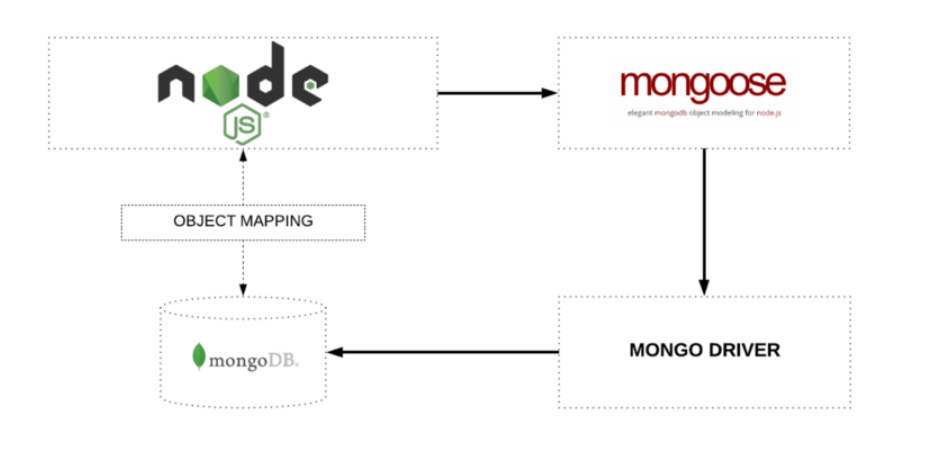
\includegraphics[width=0.8\textwidth]{./images/chapter2/mongoose.png}
	\caption[Mongoose, ένα abstract layer μεταξύ Node και mongo]
	{H mongoose λειτουργεί ώς ένα abstract layer μεταξύ της Node και των driver της mongo προκειμένου η επικοινωνία μεταξύ των δύο να γίνεται πιο εύκολα}
	\label{fig:mongoose}
\end{figure}

\break

\subsection{Google Cloud Storage}
\label{subsec:gcloud}

Πέρα από την κλασική βάση δεδομένων που προαναφέραμε θέλουμε να αποθηκεύουμε ιστορικά δεδομένα,
δεδομένα δηλαδή που δεν θα δείχνουμε άμεσα στον χρήστη, αλλά θα κρατάμε για να υπολογίζουμε μετρικές
και στατιστικά σημαντικά αποτελέσματα στο σύνολο όλης της μέχρι τώρα αποθηκευμένης πληροφορίας.

Σε αυτό λοιπόν το σημείο έρχεται το Google Cloud Storage (GCP), το οποίο παρέχει μεταξύ άλλων δυνατότητες
Αποθήκευσης Αρχείων (File Storage). Τα δεδομένα αυτά δεν χρειάζεται να υπακούουν σε κάποιο σχήμα
ενώ παράλληλα ο τρόπος αρχειοθέτησης των δεδομένων ταυτίζεται με ένα κλασικό σύστημα αρχείων
ενός υπολοσιστικού συστήματος. Διαθέτει paths και τύπους αρχείων όπως ακριβώς και οι υπολογιστές και όλες οι
συσκευές που χρησιμοποιούμε. Για να διαβάσεις κανείς πληροφορία, χρειάζεται να ξέρει μόνο το μονοπάτι που οδηγεί
στο επιθυμητό αρχείο καθώς και τη μορφή αυτού. Οι υποστηριζόμενοι τύποι αρχείων μέχρι τώρα είναι οι εξής:

\begin{itemize}
	\item Binary
	\item Flat
	\item JSON
	\item Avro
	\item Parquet
\end{itemize}

